\documentclass[11pt,a4paper]{article}
\usepackage[margin=25mm]{geometry}
\usepackage{amsmath,amssymb,amsthm,graphicx,booktabs,array,hyperref,xcolor,microtype}
\usepackage[T1]{fontenc}
\usepackage{lmodern}
\usepackage{caption}
\usepackage[section]{placeins}
\hypersetup{colorlinks=true,linkcolor=blue!45!black,citecolor=blue!45!black,urlcolor=blue!45!black}
\captionsetup{font=small,labelfont=bf}
\newtheorem{proposition}{Proposition}
\newtheorem{lemma}{Lemma}
\newcommand{\R}{\mathbb R}
\newcommand{\C}{\mathbb C}
\newcommand{\tr}{\operatorname{tr}}
\newcommand{\diag}{\operatorname{diag}}
\title{\textbf{Beyond Orbit Fit: Observation Geometry and Structural Priors\\in Learning Hopf Bifurcations}}
\author{Jiajun Fu\\Duke Kunshan University}
\date{October 14, 2026}
\begin{document}
\maketitle
\begin{abstract}
Learning a differential equation from trajectories does not automatically recover its transverse stability or bifurcation structure. We investigate this distinction through a reproducible computational study of planar oscillators. An elementary ambiguity construction shows that identical invariant-orbit observations can coexist with opposite transverse stability; corresponding polynomial dictionaries retain exact column dependencies. At matched observation counts, passive orbit sampling, random transients and small radial probes are compared using polynomial regression and trajectory-trained neural ordinary differential equations (NODEs). In a noiseless cubic benchmark, random transients give correctly directed unique candidate crossings in all five NODE initializations at each budget, whereas passive data usually fail. Small probes are highly accurate with the correct polynomial dictionary but are sensitive to observational noise; larger probes improve selected NODE controls. A non-radial FitzHugh--Nagumo experiment separates local criticality from critical-parameter accuracy: all five NODEs recover a subcritical Hopf type numerically, despite location errors between 0.0037 and 0.0855. Selected periodic orbits are checked through shooting, transverse Floquet multipliers and tolerance refinement. The results establish conditional interactions between acquisition geometry, structural priors and optimization, rather than a universally optimal sampling strategy.
\end{abstract}
\noindent\textbf{Keywords:} neural differential equations; Hopf bifurcation; identifiability; observation design; transverse stability; scientific machine learning.

\section{Introduction}
The central question of this study is:
\begin{quote}
When observations cover finite initial conditions, time horizons and parameter ranges, can learned differential equations recover bifurcation locations, equilibrium stability and attractors? Which observation designs and declared structural priors improve recovery at matched measurement budgets?
\end{quote}
A trajectory measures a vector field only along a particular path. A stability decision additionally depends on how nearby trajectories evolve. Consequently, a model can reproduce an observed oscillation while misrepresenting the dynamics normal to that oscillation. This distinction is especially important near a Hopf transition, where weak growth or decay makes short observation windows difficult to interpret.

Our objective is an original, controlled computational comparison, not a new NODE architecture. The study contributes a linked chain of evidence: an exact restricted-observation ambiguity; matched acquisition and compute experiments with explicit diagnostic failures; noise and excitation controls; and independent local and periodic-orbit checks on a non-radial system. Synthetic truth makes these checks reproducible, while also limiting claims about real experimental data. The elementary mathematical observations below are explanatory arguments and are not claimed as previously unknown theorems.

\section{Related work and positioning}
Neural ordinary differential equations represent continuous dynamics with a trainable vector field \cite{chen}. Sparse identification provides interpretable equation discovery and can incorporate parameter dependence \cite{brunton}. Vortmeyer-Kley, Nieters and Pipa study trajectory-related losses for missing-term learning across bifurcating systems \cite{vortmeyer}. Mechanistic and learned components have also been combined for experimental bifurcation analysis and Hopf oscillations \cite{beregi,lee}.

The closest comparator is van Tegelen et al.\ \cite{tegelen}, who learn parameter-dependent NODEs and investigate bifurcation extrapolation, limited data, noise and state-space coverage. Thus neither learning a bifurcation with a NODE nor the general observation that coverage matters is a novelty claim here. Our narrower emphasis is a matched-count comparison of orbit, transient and transverse-probe observations, coupled to an explicit ambiguity argument and to separate location, orientation, criticality and periodic-stability diagnostics. This paper does not reproduce every competing method or establish exhaustive literature priority.

\section{Mathematical setting and observation ambiguity}
\subsection{Reference radial systems}
Let $z=x+iy$. The principal benchmark is
\begin{equation}
 \dot z=(\mu+i)z-|z|^2z,\qquad
 \dot r=\mu r-r^3,\quad \dot\theta=1. \label{eq:hopf}
\end{equation}
The equilibrium has eigenvalues $\mu\pm i$. For $\mu>0$, the cycle radius is $r_*=\sqrt{\mu}$, its period is $2\pi$, and its transverse exponent is $-2\mu$. At $\mu=0$, attraction remains algebraic rather than exponential.
For $u=r^2$ and $u_0>0$,
\begin{equation}
u(t)=\frac{\mu}{1+(\mu/u_0-1)e^{-2\mu t}}\quad(\mu\ne0),
\qquad u(t)=\frac{u_0}{1+2u_0t}\quad(\mu=0). \label{eq:exact}
\end{equation}
These formulas provide independent numerical validation targets.

A richer reference family is
\begin{equation}
\dot z=\left[\mu-a|z|^2-b|z|^4+i(1+c|z|^2)\right]z,\quad a>0,\ b\ge0.
\end{equation}
Its positive squared cycle radius is
$s_*=2\mu/[a+\sqrt{a^2+4b\mu}]$; its transverse exponent is $-2as_*-4bs_*^2$. This family validates the reference solver, but is not used as an additional learned-model generalization result.

\subsection{Exact orbit agreement need not identify stability}
\begin{proposition}[Restricted invariant-set ambiguity]
Consider $\dot z=iz+c(\mu)(\mu-|z|^2)z$. At each observed positive parameter, all choices of $c$ generate the same motion on $|z|^2=\mu$. At each observed negative parameter, all choices produce the same constant trajectory at $z=0$. These observations alone do not determine the equilibrium growth rate or cycle transverse exponent.
\end{proposition}
\begin{proof}
On the observed circle, the radial factor is zero and $\dot z=iz$, independently of $c$. At the origin, $\dot z=0$. At the origin the real eigenvalue part is $c(\mu)\mu$. At the positive-parameter circle, differentiating $c(\mu)r(\mu-r^2)$ gives the transverse exponent $-2c(\mu)\mu$. Opposite signs of $c$ therefore reverse stability without changing the restricted observations.
\end{proof}
This construction shows a stability ambiguity, not an arbitrary shift of the Hopf point: when $c$ is smooth and nonzero near zero, its crossing remains at zero. Nor does it imply indistinguishability when additional transient validation observations are available.

For the dictionary used below, passive observations satisfy
\begin{equation}
\mu x=x^3+xy^2,\qquad \mu y=x^2y+y^3. \label{eq:dependencies}
\end{equation}
Both identities also hold at the observed negative-parameter origin. Thus at least two dictionary columns are linearly dependent, regardless of repeated sampling on these sets.

\begin{figure}[t]
\centering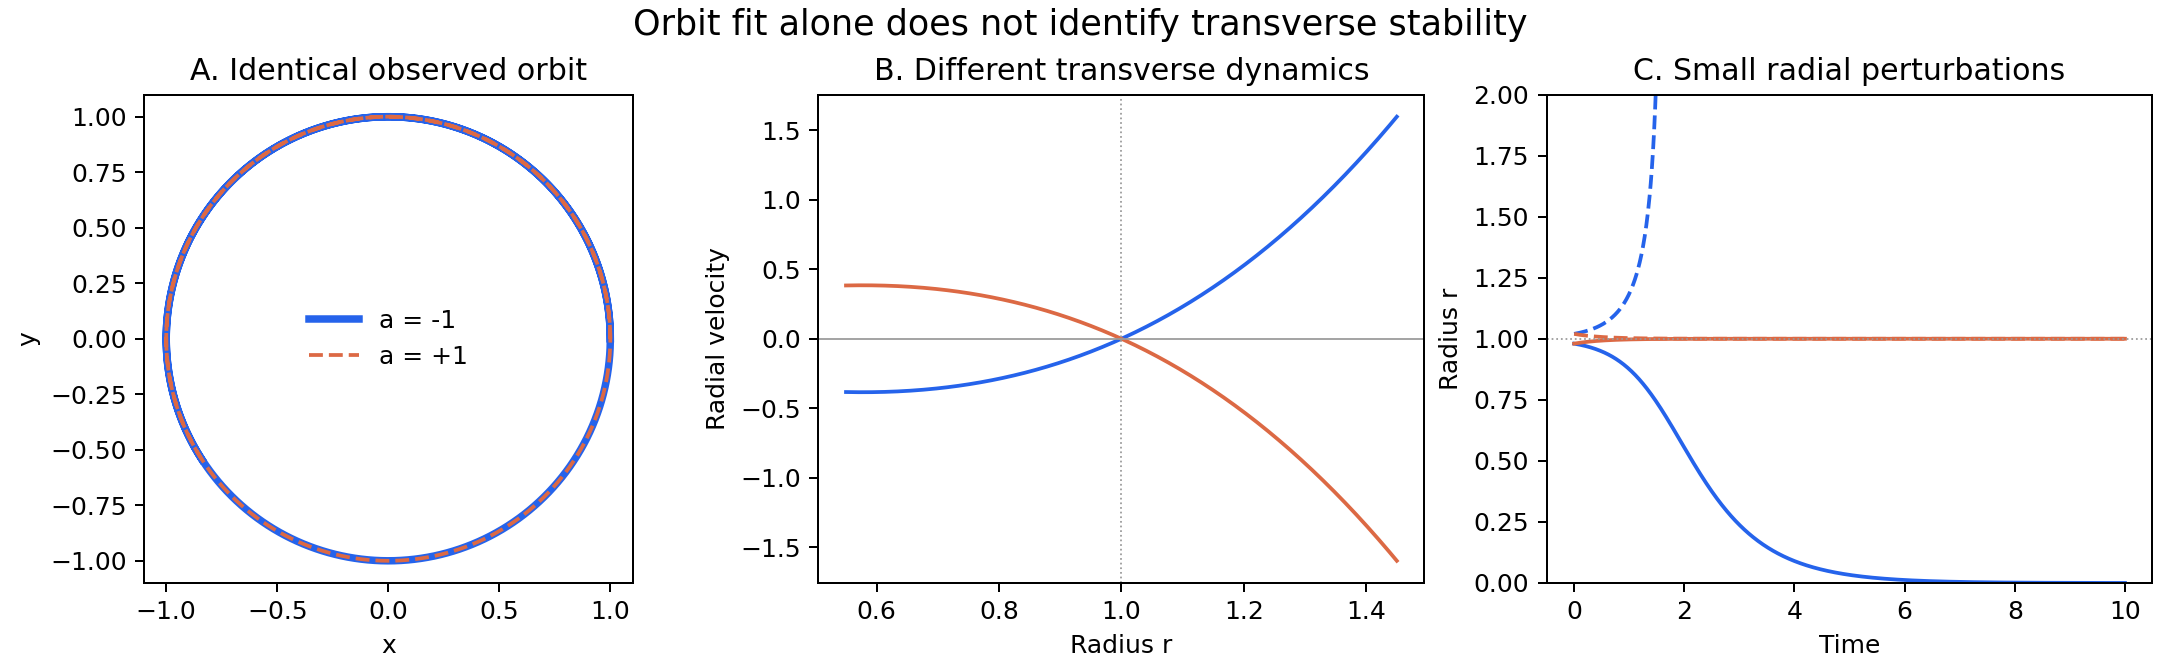
\includegraphics[width=\linewidth]{../phase0/motivation.png}
\caption{An illustrative pair $\dot r=ar(1-r^2)$, $\dot\theta=1$ has identical motion on $r=1$ but transverse exponent $-2a$. Small radial perturbations distinguish stability. This is an analytic construction, not a trained-model result.}
\end{figure}

\subsection{A conditional local accuracy statement}
Define a continuous equilibrium branch $e(\mu)$ and
$g(\mu)=\frac12\tr D_xf(e(\mu),\mu)$.
\begin{lemma}[Conditional crossing-location bound]
Suppose $g(\mu_c)=0$, $g$ is differentiable on an interval, $|g'|\ge m>0$ there, and $|\widehat g-g|\le\varepsilon$ uniformly. If $\widehat g(\widehat\mu_c)=0$ within that interval, then
$|\widehat\mu_c-\mu_c|\le\varepsilon/m$.
\end{lemma}
\begin{proof}
At the learned root, $|g(\widehat\mu_c)|\le\varepsilon$. The mean value theorem gives $g(\widehat\mu_c)-g(\mu_c)=g'(\xi)(\widehat\mu_c-\mu_c)$.
\end{proof}
Root existence, uniqueness, positive determinant and nonlinear nondegeneracy require separate checks. The bound is a standard local estimate, not a certification inferred from trajectory MSE. If $D_xf$ has Lipschitz constant $L$ near the equilibrium branch and the learned branch is displaced by $\delta_e$, then, under a uniform same-state Jacobian error $\delta_J$, the effective Jacobian error is bounded by $\delta_J+L\delta_e$. A two-dimensional trace error is at most twice its operator-norm bound. This explains why derivative and equilibrium accuracy are relevant even when orbit fit appears good.

\section{Models and numerical diagnostics}
\subsection{Polynomial and equivariant models}
The unconstrained polynomial dictionary is
\begin{equation}
\Theta=(1,x,y,\mu,\mu x,\mu y,x^2,xy,y^2,x^3,x^2y,xy^2,y^3).
\end{equation}
Each output has separate coefficients. Ordinary least squares is applied to derivatives estimated using a nine-point, degree-three Savitzky--Golay filter; four samples are removed at each endpoint. This is not sparse SINDy, and no true derivative labels are provided. The dictionary contains the true cubic equations, a substantial structural advantage.

The rotationally equivariant comparator learns all six coefficients in
\begin{equation}
\dot z=[b_0+b_1\mu+b_2|z|^2+i(c_0+c_1\mu+c_2|z|^2)]z.
\end{equation}
Its candidate threshold is $-b_0/b_1$, rather than a supplied zero. This class is a subspace of the unconstrained dictionary and is used only for radial systems.

\subsection{Trajectory-trained NODE}
The vector field is a two-hidden-layer tanh network with input $(x,y,\mu)$, width 24 and two outputs: 746 trainable parameters. Training integrates six-step segments with RK4 and minimizes
\begin{equation}
\mathcal L=\frac{1}{2KB}\sum_{j=1}^{K}\sum_{b=1}^{B}
\|\widehat{\boldsymbol x}_{b,j}-\boldsymbol x_{b,j}\|_2^2,\quad K=6,\ B=48.
\end{equation}
Reverse differentiation through RK4 is implemented explicitly in NumPy. Centered finite differences check one entry in each parameter tensor; independent differences check analytic network Jacobians. Adam uses learning rate 0.003 and gradient clipping at norm 5. Checkpoints are evaluated every 100 steps using a twelve-step validation loss. Five paired initialization seeds are used in the main comparison.

\subsection{Crossings and criticality}
At each parameter, the implemented diagnostic follows one equilibrium branch, checks the residual, evaluates its Jacobian and brackets trace-zero crossings with positive determinant. Missing or ambiguous crossings are retained as failures. Following one branch does not exclude additional equilibria elsewhere.

At selected candidates, the standard first Lyapunov coefficient \cite{kuznetsov} is computed as
\begin{align}
l_1=\frac{1}{2\omega}\Re\langle p,&C(q,q,\bar q)
-2B(q,A^{-1}B(q,\bar q))\nonumber\\
&+B(\bar q,(2i\omega I-A)^{-1}B(q,q))\rangle, \label{eq:l1}
\end{align}
where $Aq=i\omega q$, $A^\top p=-i\omega p$, $\langle p,q\rangle=1$ and $B,C$ are the second- and third-derivative multilinear forms. Eigenvectors have the declared unit normalization. Derivative steps 0.002 and 0.001 test sign consistency. Nonzero crossing slopes are checked separately.

\subsection{Periodic shooting and stability}
Set $x_0=e_x(\mu)+\rho$, $y_0=e_y(\mu)$ and solve for $(\mu,T)$ satisfying
\begin{equation}
\Phi_T(x_0,y_0;\mu)-(x_0,y_0)=0.
\end{equation}
For a closed planar autonomous orbit, the tangent Floquet multiplier is one. Liouville's formula gives the nontrivial multiplier
\begin{equation}
M_\perp=\exp\left(\int_0^T\tr D_xf(\boldsymbol x(t),\mu)\,dt\right).
\end{equation}
We classify $M_\perp<1$ as transversely stable and $M_\perp>1$ as unstable. These are selected fixed-section continuation points, not a complete global or pseudo-arclength bifurcation diagram.

\section{Experimental design}
\subsection{Main matched-count comparison}
Training parameters are $-0.4,-0.2,0.2,0.4$; validation parameters are $-0.3,0.3$; test parameters are $-0.1,0.1$. Whole trajectories are split; adjacent time points are never split between training and test. This is interpolation across a withheld critical band.

Every trajectory has 64 full-state observations over $T=5$, costing 128 scalar measurements. Budgets 4096 and 16384 give 32 and 128 training trajectories, equally divided over the four parameters. Validation and test each cost 1024 scalar observations. The larger budget adds initial conditions, not new parameters or longer observation windows.

Passive trajectories start at $r=0$ for negative $\mu$ and $r=\sqrt{\mu}$ for positive $\mu$. Random transients use uniform radii in $[0.05,0.8]$. Probes displace positive-parameter anchor radii by $\pm0.02$ and negative-parameter origins by radius 0.02; phases are random. All repeated zero observations count toward the measurement budget; unique-state counts are recorded separately.

The acquisition process knows the true attractor anchors, but the learners receive only states and parameter labels. Anchor search, settling and physical intervention costs are excluded. Thus the comparison is conditional on anchor access, not an end-to-end cost study.

Paired initialization seeds and optimizer seeds are matched across designs. Each NODE trains to 3600 steps, with evaluations at 1200 and 3600 using the best validation checkpoint within each cap. Full validation histories and balanced training-segment losses are retained. Matching compute and extending training control effort but do not prove convergence.

\begin{figure}[t]
\centering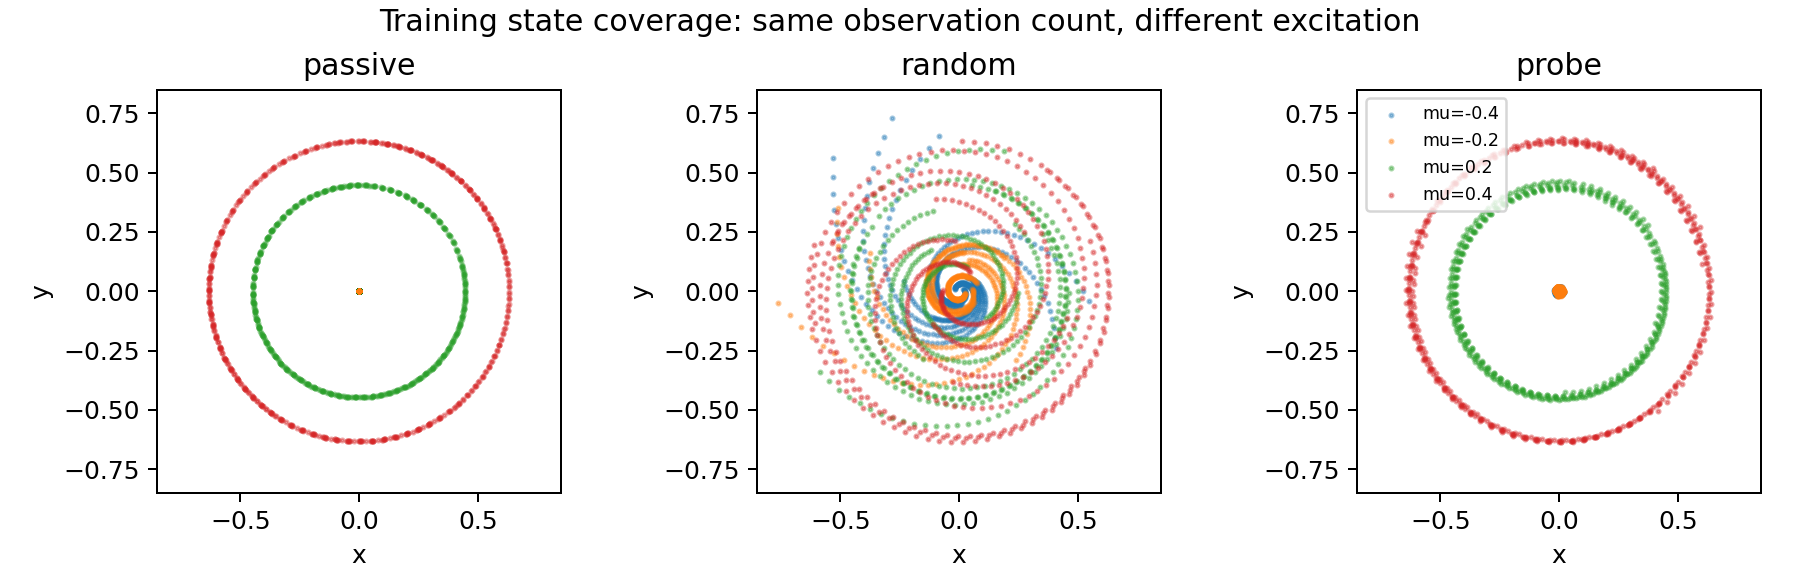
\includegraphics[width=\linewidth]{../phase3/training_coverage.png}
\caption{Training-state coverage at 4096 scalar observations. Passive data occupy invariant sets; random transients span a broader region; small probes occupy narrow neighborhoods. Colors identify the four training parameters.}
\end{figure}

\subsection{Robustness and replication}
Polynomial experiments vary probe radius $0.005,0.02,0.1$, window $T=5,20$, and absolute Gaussian observation-noise standard deviation $0,0.01,0.05$, with five acquisition seeds. The passive and random designs each use one nominal probe setting. This yields 150 fits per polynomial model class.

Twenty additional unconstrained polynomial fits use only negative training parameters $[-0.4,-0.3,-0.2,-0.1]$. Selected NODE controls comprise six acquisition/noise/window settings, two acquisition seeds and two initialization seeds: 24 runs. Their common validation set is clean and contains 1024 scalar observations. This idealizes noisy validation and is stated explicitly.

Keeping 64 samples when $T$ increases coarsens sampling and lengthens physical training segments. Consequently, the duration control does not isolate the effect of observing longer. Noise affects observed states as well as estimated derivatives; errors-in-variables and filtering biases are not removed by this protocol.

\section{Results on the radial benchmark}
\subsection{Prediction and crossing recovery}
The preliminary learning experiment uses 2048 scalar training observations. Across five NODE seeds, short held-out trajectory MSE ranges from $2.20\times10^{-4}$ to $1.19\times10^{-3}$, while candidate threshold errors range from 0.0260 to 0.1736. Seed 4 has lower trajectory MSE than seed 3 but larger crossing error, demonstrating that the two criteria need not rank models identically in this pilot.

The main matched-count results are shown in Table~\ref{tab:main}. Conditional medians must always be interpreted alongside failure counts. An error based on one successful run is not a robust aggregate estimate.
\begin{table}[tb]
\centering\small
\caption{Main NODE comparison at 3600 steps. Candidate counts and conditional median errors are both reported.}\label{tab:main}
\begin{tabular}{rlrr}\toprule
Budget & Design & Unique candidates & Median error \\
\midrule
4096 & Passive & 1/5 & 0.263624 \\
4096 & Random & 5/5 & 0.027710 \\
4096 & Probe & 3/5 & 0.159920 \\
16384 & Passive & 1/5 & 0.264990 \\
16384 & Random & 5/5 & 0.045078 \\
16384 & Probe & 2/5 & 0.269918 \\
\bottomrule\end{tabular}
\end{table}


\begin{figure}[t]
\centering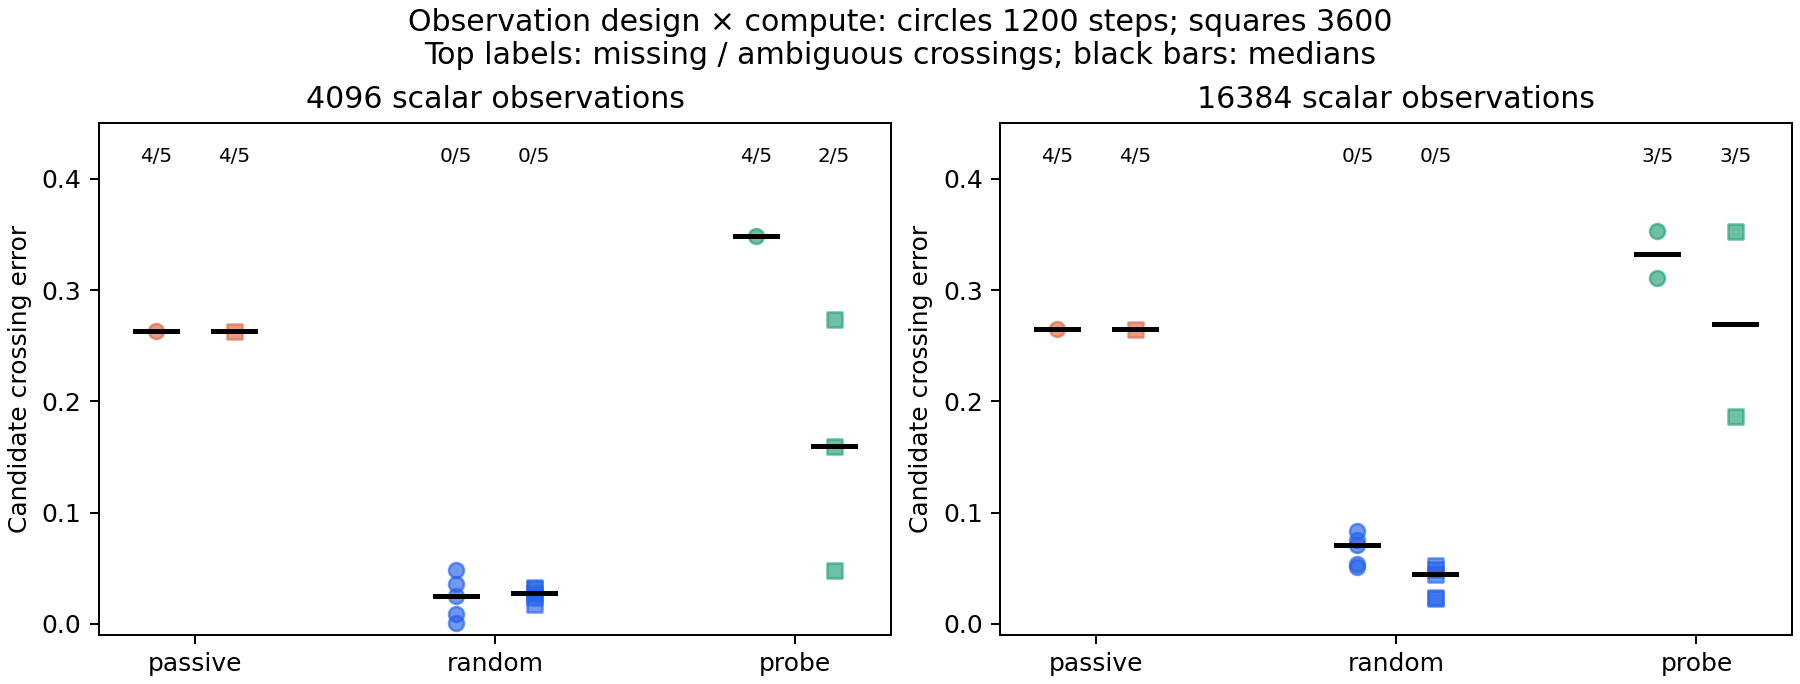
\includegraphics[width=\linewidth]{../phase3/design_comparison.png}
\caption{Every main-comparison candidate error at both compute caps. Circles: 1200 steps; squares: 3600. Top labels count missing/ambiguous candidates; black bars indicate conditional medians. No failed run is imputed as zero.}
\end{figure}

Passive polynomial matrices have rank 11/13 at both budgets, consistent with Eq.~\eqref{eq:dependencies}. Random and probe matrices have rank 13/13. At budget 4096, their smallest singular values are 0.5892 and 0.0607, respectively, using the same unscaled dictionary. These values describe conditioning under this feature scaling, not a coordinate-invariant information measure.

With the correct polynomial dictionary, probes recover the threshold to about $1.3\times10^{-7}$ at both budgets; random data yield errors $2.39\times10^{-5}$ and $1.38\times10^{-5}$. The passive polynomial diagnostic cannot recover a reliable crossing and flags many roots; numerical failure alone is not an identifiability proof, which is supplied separately by the restricted-set argument.

At 4096 observations and 3600-step selection, median balanced training-segment losses are $4.44\times10^{-6}$, $3.79\times10^{-6}$ and $2.26\times10^{-6}$ for passive, random and probe designs. Thus relative training loss alone does not explain the probe group's poor generalization. Architecture, conditioning and optimization can all contribute.

\subsection{Noise, amplitude and structural priors}
\begin{table}[tb]
\centering\small
\caption{Unconstrained polynomial noise sensitivity at $T=5$: candidate error medians over five acquisition seeds. Every displayed cell has five unique candidates.}\label{tab:noise}
\begin{tabular}{lrrr}\toprule
Design & $\sigma=0$ & $\sigma=0.01$ & $\sigma=0.05$ \\
\midrule
Random & 1.33e-05 & 0.00192 & 0.04583\\
Probe 0.005 & 4.75e-09 & 0.01148 & 0.09412\\
Probe 0.02 & 1.07e-07 & 0.00305 & 0.08271\\
Probe 0.10 & 1.75e-06 & 0.00231 & 0.02366\\
\bottomrule\end{tabular}
\end{table}

Table~\ref{tab:noise} shows the unconstrained polynomial's noise sensitivity. Without noise, tiny probes exploit local structure effectively. At noise standard deviation 0.01, the smallest probe's median error increases by several orders of magnitude. A larger probe sacrifices some noiseless precision but is more robust in these noisy cells.

The equivariant comparator improves some noise cells: at $T=5,\sigma=0.01$, random and radius-0.02 probe medians become 0.00134 and 0.00193, compared with 0.00192 and 0.00305 for the unconstrained dictionary. Radius-0.10 probes do not improve in the same comparison. A declared prior therefore has conditional, rather than uniform, benefits.

\begin{figure}[t]
\centering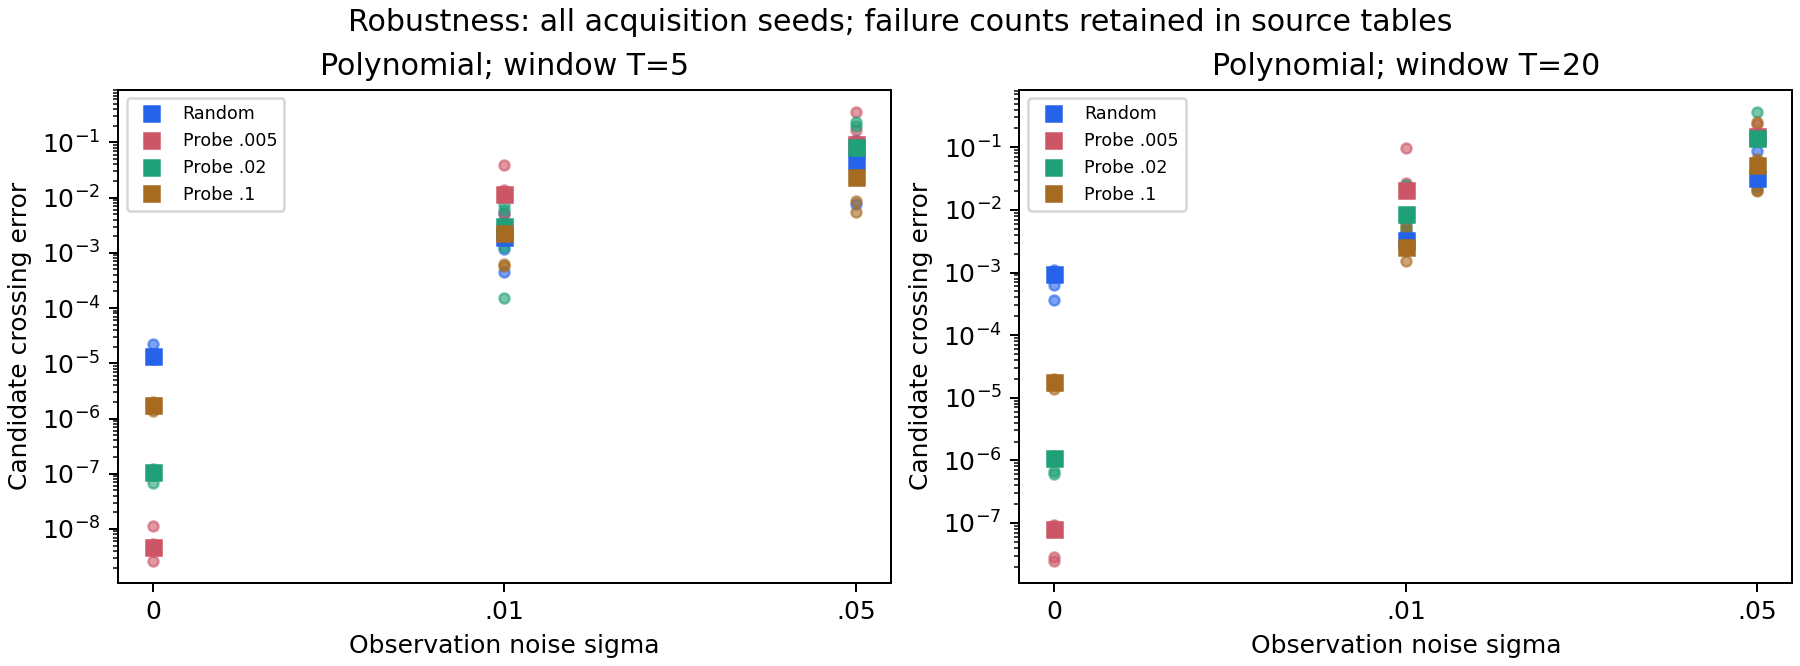
\includegraphics[width=\linewidth]{../phase4/polynomial_sensitivity.png}
\caption{Polynomial noise sensitivity across acquisition seeds. Squares indicate medians of recovered candidates. Failure and orientation counts for every cell, including passive cells, remain in the accompanying source tables.}
\end{figure}

In replicated NODE controls, noiseless random transients yield correctly directed unique crossings in 4/4 runs, small radius-0.02 probes in 0/4, and radius-0.10 probes in 4/4. The small-probe group has one unique crossing with the wrong orientation. Larger excitation improves consistency here, but its median error 0.08315 still exceeds the random group's 0.03739. Four outcomes combine two data seeds and two model seeds and are not four independent data replicates.

For one-sided polynomial extrapolation, random-data median error is $4.03\times10^{-5}$ noiseless and 0.00617 at $\sigma=0.01$. Noisy small probes recover four of five candidates with conditional median 0.12258. Because the correct cubic dictionary is supplied, these outcomes do not establish prior-free or NODE extrapolation.

\section{Non-radial validation and periodic structure}
\subsection{FitzHugh--Nagumo reference}
We use a standard planar excitable-system form \cite{fitzhugh,nagumo}:
\begin{equation}
\dot x=x-x^3/3-y+I,\qquad \dot y=\epsilon(x+\alpha-\beta y),
\quad(\epsilon,\alpha,\beta)=(0.08,0.7,0.8).
\end{equation}
The equilibrium satisfies
\begin{equation}
y_*=(x_*+\alpha)/\beta,\quad
I=(x_*+\alpha)/\beta-x_*+x_*^3/3,
\end{equation}
whose derivative $1/\beta-1+x_*^2$ is positive. The equilibrium branch is unique. Its Jacobian is
\begin{equation}
J=\begin{pmatrix}1-x_*^2&-1\\ \epsilon&-\epsilon\beta\end{pmatrix},
\quad \tr J=1-x_*^2-\epsilon\beta,\quad
\det J=\epsilon(1-\beta+\beta x_*^2)>0.
\end{equation}
For the lower-current crossing,
$x_H=-\sqrt{1-\epsilon\beta}$ and $I_H=0.33128133745$.
The frequency is 0.27550680572 and
\begin{equation}
\frac{d\,\Re\lambda}{dI}\bigg|_{I_H}
=-\frac{x_H}{1/\beta-1+x_H^2}=0.81574277386>0.
\end{equation}
The first Lyapunov coefficient is positive, $l_1=0.97197108199$ under the declared normalization, supporting subcritical local type.

\subsection{Learning and independent checks}
Training currents are $[0.12,0.22,0.44,0.54]$, validation $[0.18,0.48]$ and test $[0.30,0.36]$. Thirty-two training trajectories, each with 128 full-state samples over $T=20$, cost 8192 scalar observations. Validation and test each cost 2048. Initial states are uniformly sampled from $x\in[-2,2]$, $y\in[-0.5,1.5]$, without equilibrium anchors. NODE normalization uses training statistics only.

The polynomial candidate is 0.32959536268, an error of 0.00168597. NODE errors range from 0.00371 to 0.08549 (Table~\ref{tab:fhn}). All five have positive crossing slopes and positive Lyapunov coefficients, numerically preserving subcritical type while shifting location. This validates non-radial learning and diagnostics, not the three-way acquisition ranking on this system.
\begin{table}[tb]
\centering\small
\caption{FHN learned critical currents and physical-coordinate test MSE over $T=20$. True current $I_H=0.33128133745$. All entries recover one candidate crossing.}\label{tab:fhn}
\begin{tabular}{lrrr}\toprule
Model & Candidate current & Location error & Test MSE \\
\midrule
Polynomial & 0.329595 & 0.001686 & 4.93e-06 \\
NODE seed 0 & 0.380412 & 0.049131 & 0.0236 \\
NODE seed 1 & 0.334996 & 0.003715 & 0.0283 \\
NODE seed 2 & 0.399917 & 0.068635 & 0.0367 \\
NODE seed 3 & 0.416776 & 0.085495 & 0.0287 \\
NODE seed 4 & 0.263093 & 0.068188 & 0.034 \\
\bottomrule\end{tabular}
\end{table}


\begin{figure}[t]
\centering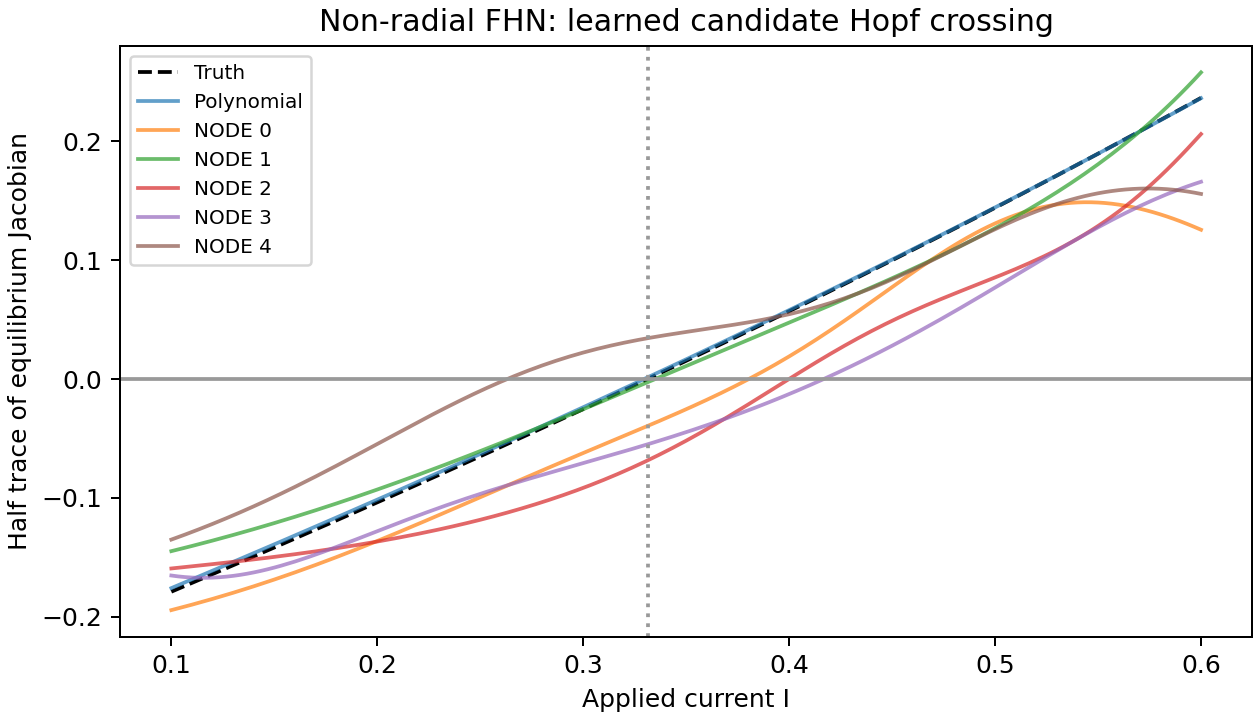
\includegraphics[width=.9\linewidth]{../phase4/fhn_crossings.png}
\caption{FHN equilibrium-branch crossing functions. Several NODEs reproduce local qualitative type while substantially shifting the critical current. Root diagnostics follow one branch and do not certify absence of other equilibria.}
\end{figure}

Five selected radial NODEs have negative coefficients and positive crossing slopes. Selected radial cycles are stable, whereas nearby FHN cycles are unstable. Twenty-one shooting points pass tolerance refinement; the largest tighter closing error is $2.48\times10^{-10}$. One FHN NODE section point fails and remains recorded. It is not interpreted as evidence of a fold or disappearance.

\begin{figure}[t]
\centering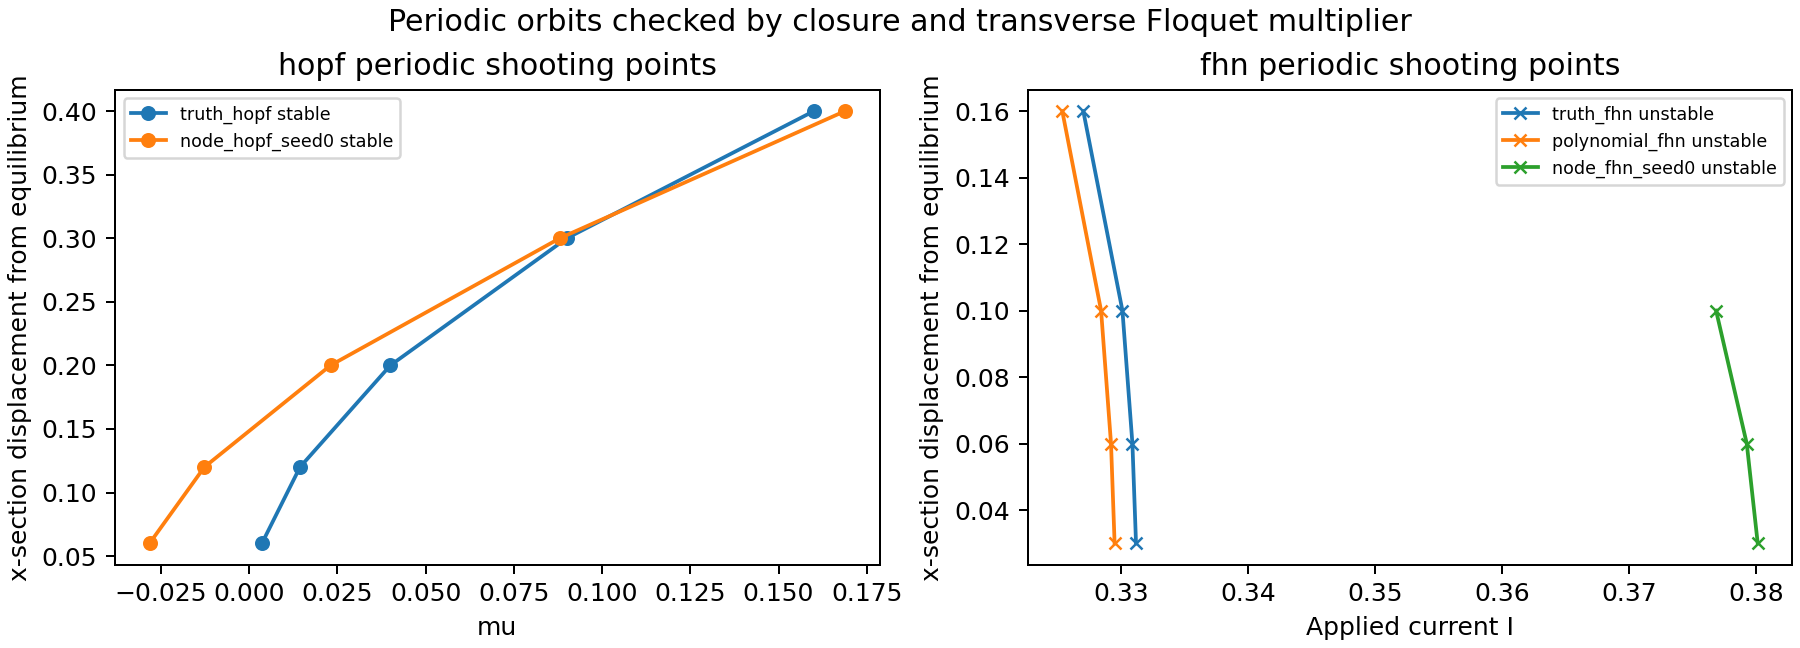
\includegraphics[width=\linewidth]{../phase4/periodic_branches.png}
\caption{Selected periodic shooting points, with stability determined by transverse Floquet multipliers. Section displacement is not a coordinate-invariant amplitude. Connected points do not constitute a full global continuation diagram.}
\end{figure}

\section{Discussion and limitations}
The observations support a bounded interaction between acquisition and model class. Exact orbit data omit transverse information in the constructed benchmark. Random transients provide broad excitation for the unconstrained NODE; small probes can suffice for a correct dictionary but become vulnerable to noise and weak sensitivity. The data-count increase does not repair exact passive dependencies, and more data at fixed compute do not monotonically improve NODE candidate accuracy.

The following limits matter for interpretation. First, synthetic equations and a correct polynomial dictionary favor interpretable regression. Second, radial acquisition uses oracle anchors and excludes setup costs. Third, clean validation for noisy NODE training is an optimistic idealization. Fourth, the duration control couples window, sampling and segment length. Fifth, five initialization seeds or two acquisition seeds provide limited uncertainty characterization; no population-level superiority test is claimed. Sixth, matched training effort does not establish convergence, and optimization-related mechanisms are not isolated causally. Finally, only local criticality and selected periodic branches are checked. Global folds, complete attractor maps, real data, latent states and stochastic forcing remain outside scope.

The original contribution is the reproducible combination of these controlled experiments and diagnostics. It is not a universal algorithm, a new identifiability theorem or a priority claim for bifurcation learning.

\section{Conclusion}
Finite observation design affects what a learned differential equation can recover beyond orbit fit. In the tested radial systems, passive invariant-set observations remain insufficient for transverse identification; broader transients and declared structure change recovery substantially. Very small probes lose their noiseless advantage under observation noise. On a non-radial system, models can preserve local Hopf type while misplacing the transition. Evaluating location, direction, nonlinear criticality and periodic stability separately produces a more informative assessment than trajectory error alone.

\section*{Reproducibility and computational assistance}
All data are synthetic and generated by the supplied scripts. The repository contains saved model weights, acquisition arrays, full seed results, failed diagnostics, numerical checks, rendering metadata and an offline interactive demo. Training uses NumPy/SciPy rather than a deep-learning runtime. Independent adaptive integration evaluates the RK4-trained vector fields. Reference dependencies and command ordering are documented in the README and reproduction script.

This manuscript and computational implementation were developed with AI-assisted drafting and coding. Authorship, interpretation and any future submission require the named author's review. No peer-review, external experimental validation or journal acceptance is asserted.

\appendix
\section{Numerical verification details}
The reference Hopf squared-radius maximum error is $2.64\times10^{-10}$ relative to Eq.~\eqref{eq:exact}. Tightened tolerances change reference Hopf states by $8.15\times10^{-10}$ and FHN states by $5.57\times10^{-9}$. The FHN analytic and numerical trace roots agree to machine precision. Explicit RK4-gradient checks and Jacobian finite differences are stored in the audit files.

Periodic shooting uses DOP853 with relative/absolute tolerances $10^{-9}/10^{-11}$; independent refinement uses $10^{-11}/10^{-13}$. The local coefficient calculation agrees with known reference values and uses two finite-difference scales. Numerical support for nondegeneracy is distinct from a rigorous interval certificate.

\section{Visual presentation and animations}
The package includes animations of fixed-parameter Hopf trajectories, transverse probes, learned dynamics and acquisition geometry. The rendered showcase uses actual ODE particle paths with dark backgrounds, age-colored trails and Gaussian bloom. Color, brightness and particle density are presentation effects, not energy, probability or uncertainty measures. The two clocks differ and are labeled. The FHN showcase scales its axes differently; quantitative evidence uses conventional plots and arrays.

\begin{figure}[ht]
\centering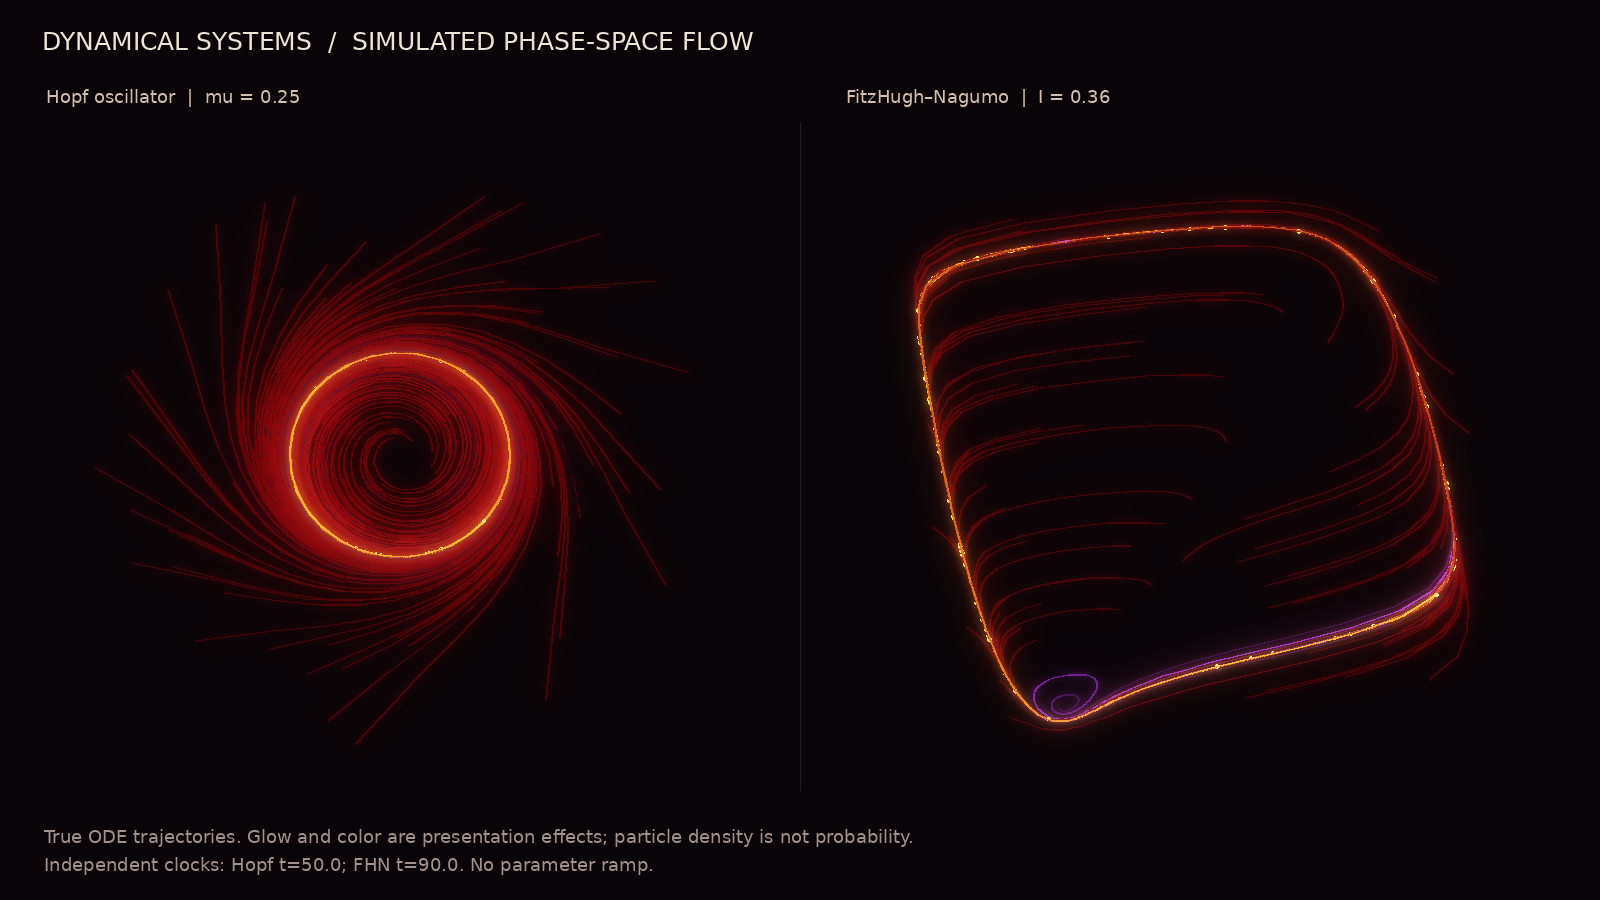
\includegraphics[width=\linewidth]{../phase4/rendered_phase_flow.png}
\caption{Showcase rendering from true phase-space trajectories. Left: Hopf $\mu=0.25$; right: FHN $I=0.36$. This image illustrates dynamics but is not a quantitative diagnostic. Animated MP4/GIF and source arrays accompany the paper.}
\end{figure}

\clearpage
\begin{thebibliography}{99}
\bibitem{chen} R. T. Q. Chen, Y. Rubanova, J. Bettencourt and D. Duvenaud. Neural ordinary differential equations. \emph{NeurIPS}, 2018. \url{https://arxiv.org/abs/1806.07366}.
\bibitem{brunton} S. L. Brunton, J. L. Proctor and J. N. Kutz. Discovering governing equations from data by sparse identification of nonlinear dynamical systems. \emph{PNAS}, 113(15), 3932--3937, 2016. \url{https://doi.org/10.1073/pnas.1517384113}.
\bibitem{vortmeyer} R. Vortmeyer-Kley, P. Nieters and G. Pipa. A trajectory-based loss function to learn missing terms in bifurcating dynamical systems. \emph{Scientific Reports}, 2021. \url{https://doi.org/10.1038/s41598-021-99609-x}.
\bibitem{beregi} S. Beregi, D. A. W. Barton, D. Rezgui and S. A. Neild. Using scientific machine learning for experimental bifurcation analysis of dynamic systems. \emph{Mechanical Systems and Signal Processing}, 184, 109649, 2023. \url{https://arxiv.org/abs/2110.11854}.
\bibitem{lee} K. Lee, D. A. W. Barton and L. Renson. Modelling of physical systems with a Hopf bifurcation using mechanistic models and machine learning. \emph{Mechanical Systems and Signal Processing}, 191, 110173, 2023. \url{https://arxiv.org/abs/2209.06910}.
\bibitem{tegelen} E. van Tegelen, G. van Voorn, I. N. Athanasiadis and P. van Heijster. Neural ordinary differential equations for learning and extrapolating system dynamics across bifurcations. \emph{Chaos}, 35, 101103, 2025. \url{https://doi.org/10.1063/5.0288264}.
\bibitem{kuznetsov} Y. A. Kuznetsov. Andronov--Hopf bifurcation. \emph{Scholarpedia}, 1(10), 1858, 2006. \url{https://doi.org/10.4249/scholarpedia.1858}.
\bibitem{fitzhugh} R. FitzHugh. Impulses and physiological states in theoretical models of nerve membrane. \emph{Biophysical Journal}, 1(6), 445--466, 1961. \url{https://doi.org/10.1016/S0006-3495(61)86902-6}.
\bibitem{nagumo} J. Nagumo, S. Arimoto and S. Yoshizawa. An active pulse transmission line simulating nerve axon. \emph{Proceedings of the IRE}, 50(10), 2061--2070, 1962. \url{https://doi.org/10.1109/JRPROC.1962.288235}.
\end{thebibliography}
\end{document}
